% ==========================================
% Document Class: APA 7th Edition for Students
% ==========================================
\documentclass[stu, floatsintext, 12pt, a4paper, donotrepeattitle]{apa7}

% ==========================================
% Packages for Graphics and Tables
% ==========================================
\usepackage{graphicx} % Required for inserting images
\usepackage{multirow} % Allows multi-row cells in tables
\usepackage{svg} % Allows inclusion of SVG images
\usepackage{tikz}
\usepackage{pgfplots}
\usetikzlibrary{intersections}
\usetikzlibrary{patterns}
\usepgfplotslibrary{fillbetween}
\pgfplotsset{compat=1.18}


% ==========================================
% Short Title for Header
% ==========================================
\shorttitle{Your short title goes here}

% ==========================================
% Custom Commands for APA-style Statistics
% ==========================================
\newcommand{\acite}[1]{{\citeauthor{#1} (\citeyear{#1})}} % Cite with author and year
\newcommand{\msd}[2]{($M$ = {#1}, $SD$ = {#2})} % Mean and Standard Deviation formatting
\newcommand{\chitest}[3]{$\chi^2$ (#2) = {#1}, $p$ ${#3}$} % Chi-square test formatting
\newcommand{\maineffect}[5]{$F$({#1}, {#2}) = {#3}, $p$ ${#4}$, $\eta^2_p$ = {#5}} % ANOVA main effect formatting
\newcommand{\levenes}[4]{$F$({#1}, {#2}) = {#3}, $p$ = {#4}} % Levene's test formatting
\newcommand{\ttest}[4]{$t$({#1}) = {#2}, $p$ ${#3}$, $d$ = {#4}} % t-test formatting
\newcommand{\shapiro}[2]{$W$ = {#1}, $p$ = {#2}} % Shapiro-Wilk test formatting

% ==========================================
% Section and Subsection Formatting
% ==========================================
\let\paragraph\oldparagraph
\let\subparagraph\oldsubparagraph
\usepackage{titlesec, blindtext, color} % Control section and subsection formatting
\titleformat{\subsubsection}[runin]{\bfseries}{\hspace{.5in}\thesubsubsection \ }{0in}{}[]
\titleformat{\subsection}[block]{\bfseries}{\thesubsection \ }{0in}{}[]
\titleformat{\section}[block]{\hfil\bfseries}{\thesection \ }{0in}{}[]

% ==========================================
% Epigraphs and Quotes
% ==========================================
\usepackage{epigraph} % For quotes at the beginning of chapters/sections
\setlength\epigraphwidth{\textwidth} % Makes epigraph span full text width
\setlength\epigraphrule{.5pt} % Sets a small horizontal rule below the quote
\usepackage{csquotes} % Provides better control over quotation marks

% ==========================================
% Table of Contents Formatting
% ==========================================
\setcounter{secnumdepth}{3} % Enables numbering up to subsubsections
\usepackage[titles]{tocloft} % Customization of table of contents
\renewcommand{\cftsecfont}{\normalsize} % Standardizes section font size in ToC
\renewcommand{\cftsecpagefont}{\normalsize} % Standardizes section page font in ToC
\renewcommand{\cftsecleader}{\cftdotfill{.}} % Adds dots to section titles in ToC
\renewcommand{\cftsubsecleader}{\cftdotfill{.}} % Adds dots to subsection titles in ToC
\renewcommand{\cftsubsubsecleader}{\cftdotfill{.}} % Adds dots to subsubsection titles in ToC
\cftsetindents{section}{0em}{1em}
\cftsetindents{subsection}{2em}{2em}
\cftsetindents{subsubsection}{3em}{3em}

% ==========================================
% General Formatting and Layout
% ==========================================
\usepackage{geometry} % Controls page margins
\geometry{margin=1in} % Sets 1-inch margins
\usepackage{makecell} % Allows thick cell borders in tables
\usepackage[document]{ragged2e} % Justifies paragraphs while keeping line breaks
\setlength{\JustifyingParindent}{.5in} % Adjusts paragraph indentation
\usepackage[activate={true,nocompatibility},final,kerning=true,spacing=false,tracking=true]{microtype} % Enhances text spacing and hyphenation
\microtypecontext{spacing=nonfrench}
\hypersetup{hidelinks} % Hides hyperlinks' colors in the table of contents

% ==========================================
% Bibliography and Referencing
% ==========================================
\usepackage[style=apa, backend=biber]{biblatex} % Uses APA-style references with Biber
\addbibresource{references.bib} % Loads the bibliography file

% ==========================================
% Fonts and Typography
% ==========================================
%\usepackage{mathptmx} % Uses Times New Roman font
\renewcommand{\arraystretch}{1.5} % Adjusts table row spacing

% ==========================================
% Miscellaneous Packages
% ==========================================
\usepackage{lipsum} % Provides placeholder text for testing
\usepackage{setspace} % Allows manual line spacing adjustments
\usepackage{amsmath} % Enhances mathematical notation

\begin{document}
\onehalfspacing
\justifying
\vspace*{4\baselineskip}
\thispagestyle{empty}
\begin{center}
   Titel Zeile 1\\Titel Zeile 2 \\
    \vspace*{5\baselineskip}
    \textbf{Bachelor Thesis} \\
    \vspace*{2\baselineskip}
    zur Erlangung des akademischen Grades \\
Bachelor of Science (B.Sc.) Psychologie \\
durch die Fakultät für Human- und Sozialwissenschaften der \\
Universitätsname \\
\vspace*{4\baselineskip}
\end{center}
vorgelegt von \\
\noindent Vor- und Nachname\\
\noindent \hspace{.5in} Straße \\
\noindent\hspace{.5in} PLZ, Ort \\
\noindent Matrikelnummer: 123456 \\
\noindent E-Mail: name@uni.de \\
\noindent Datum: 26. April 2025 \\
\begin{tabbing}
     \hspace*{1cm}\=\hspace*{1.5in}\=\hspace*{4cm}\=\hspace*{2.7cm}\= \kill
     Prüfer/in und Betreuer: \> \> Prof. Dr. Max Mustermann \\
     Prüfer/in: \> \>  Dr. Maria Musterfrau
\end{tabbing}
\section*{Abstract}
\noindent Your abstract goes here, around 250 words.
\newpage

\tableofcontents

\newpage
\section{Theoretischer Hintergrund}
\say{Test}.
\section{Methodology}
\subsection{Tables}
Tables are vital for any thesis. While \LaTeX\ does not offer the same ease in mocking up tables quickly, the tables turn out much neater and less often destroy your layout than in Word or similar programs. Writing the tables entirely by hand is not recommended, it is much faster and more seamless to use online \LaTeX\ table generation sites. Then just copy the code here and customize.  

Note, that tables in APA7 should use horizontal lines sparingly and avoid vertical lines entirely. The APA7 documentclass numbers the tables automatically and the captions and tablenotes are italized as required. This is what a table in APA7 style can look like:

\begin{table}[h]
    \caption{Descriptive characteristics of experimental groups on Big5 factors}
\label{big5}
    \begin{tabular}{lcc}
    \hline
     \textbf{Factor}& \multicolumn{2}{c}{\textit{\textbf{M {[}SD{]}}}} \\ \hline
     & Group A & Group B \\
    Agreeableness & 7.13 {[}2.11{]} & 10.95 {[}1.74{]} \\
    Extraversion & 3.54 {[}0.54{]} & 2.22 {[}4.87{]} \\
    Openness & 4.33 {[}6.32{]} & 1.64 {[}3.22{]} \\
    Neuroticism & 2.59 {[}3.99{]} & 5.66 {[}1.16{]} \\
    Concioussness & 3.88 {[}1.04{]} & 3.32 {[}4.38{]} \\ \hline
    \end{tabular}
    \tablenote{Data are made up.}
    \end{table}
\section{Results}
\subsection{Figures}
\subsubsection{Mathematical Figures}
Because the primary usecase for \LaTeX\ is the usage in natural sciences and STEM subjects, there are features to display complex mathematical illustrations. 

\begin{figure}
    \caption{Visualization of a normal distribution with the 95\% confidence interval shaded in blue and rejection regions in red.}
    \centering
    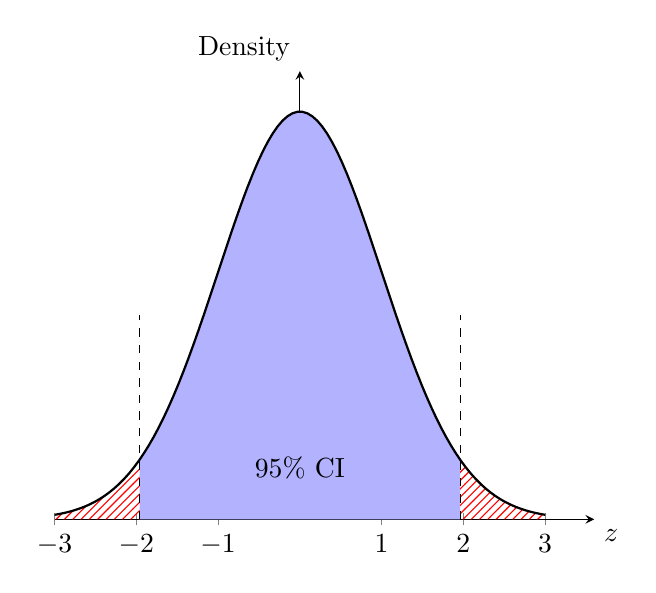
\begin{tikzpicture}
        \begin{axis}[
            axis lines=middle,
            enlargelimits=upper,
            domain=-3:3,
            samples=100,
            xtick={-3,-2,-1,0,1,2,3},
            xticklabels={$-3$,$-2$,$-1$,$0$,$1$,$2$,$3$},
            ytick=\empty,
            xlabel={$z$},
            ylabel={Density},
            every axis x label/.style={at={(current axis.right of origin)},anchor=north west},
            every axis y label/.style={at={(current axis.above origin)},anchor=south east}
        ]
        
        % Normal distribution curve
        \addplot[name path=N, domain=-3:3, samples=100, thick] {exp(-x^2/2)/sqrt(2*pi)};
        
        % Confidence interval (shaded region between -1.96 and 1.96)
        \path[name path=lower] (-1.96,0) -- (1.96,0);
        \addplot[blue!30] fill between[of=N and lower, soft clip={domain=-1.96:1.96}];
        
        % Left and right rejection regions
        \path[name path=left] (-3,0) -- (-1.96,0);
        \path[name path=right] (1.96,0) -- (3,0);
        \addplot[red!50, pattern=north east lines, pattern color=red] fill between[of=N and left, soft clip={domain=-3:-1.96}];
        \addplot[red!50, pattern=north east lines, pattern color=red] fill between[of=N and right, soft clip={domain=1.96:3}];
        
        % Vertical dashed lines for z = -1.96 and z = 1.96
        \addplot[dashed] coordinates {(-1.96,0) (-1.96,0.2)};
        \addplot[dashed] coordinates {(1.96,0) (1.96,0.2)};
        
        % Labels
        \node[anchor=north] at (axis cs:-1.96,0) {$-1.96$};
        \node[anchor=north] at (axis cs:1.96,0) {$1.96$};
        \node at (axis cs:0,0.05) {95\% CI};
        
        \end{axis}
    \end{tikzpicture}
    \label{fig:confidence_interval}
\end{figure}
\newpage
\subsubsection{External Figures}
External image files like .png or .jpg images can easily be added and automatically numbered as well. Note that the image file should be in the project folder to refer to it.

\begin{figure}
    %\centering
     \caption{An example figure}
     \includegraphics[width=\linewidth]{Tables & Figures/DCTplot.jpg}
     
     %\label{fig:enter-label}
 \end{figure}
\include{discussion}
\newpage

\newpage
\section{References}
\printbibliography[heading=none]

\appendix
\newpage
\addcontentsline{toc}{section}{Appendix}
\section{Additional material}
If there is one section in the appendix, the appendix is not enumerated. However, if you add another section to the appendix, they are then labeled alphabetically.


\newpage
\newpage
\begin{center}
    \noindent \large\textbf{Eigenständigkeitserklärung}
\end{center}

\vspace{1cm}
\noindent Ich, YOUR NAME, erkläre hiermit, dass diese Abschlussarbeit mit dem Titel „[Thesis Title]“ meine eigene Arbeit ist. Ich habe keine anderen Quellen, Hilfsmittel oder Unterstützung verwendet als die ausdrücklich im Text angegebenen.\vspace{.3cm}

\noindent Alle von mir zitierten, paraphrasierten oder anderweitig verwendeten Quellen sind ordnungsgemäß angegeben. Diese Arbeit entspricht den Richtlinien zur wissenschaftlichen Integrität der [University Name].

\vspace{35mm}
\begin{tabular}{@{}p{2in}p{3.5in}@{}}
Stadt, 26. April 2025 & \hrulefill\\
& \centering Ihr Vor- und Nachname \\
\end{tabular} 


\end{document}
